%=======================================================================
% Copyright (c) 2012 The University of York and Willink Transformations.
%
% $Id: motivation.tex 5454 2013-05-17 09:47:03Z hhoyos@CS.YORK.AC.UK $
%=======================================================================
\section{Motivation}\label{sec:motivation}

A \textit{model transformation} is the automated maintenance of a set of target models from a set of source models \cite{Kleppe.etal2003}. The models comprise Objects that are instances of Types within Packages, all defined by metamodels. As shown in Figure \ref{fig:TransformationAnatomy}, a declarative transformation defines relationships between the models by specifying mappings (or rules) between the left and right metamodel elements. Each mapping relates a Pattern of left Objects to a Pattern of right Objects. When the transformation executes, the Patterns are instantiated as Bindings in which each Binding identifies the Object in use for each Pattern element. The set of all possible distinct Bindings forms the execution trace.

\begin{figure}[h]
	\centering
	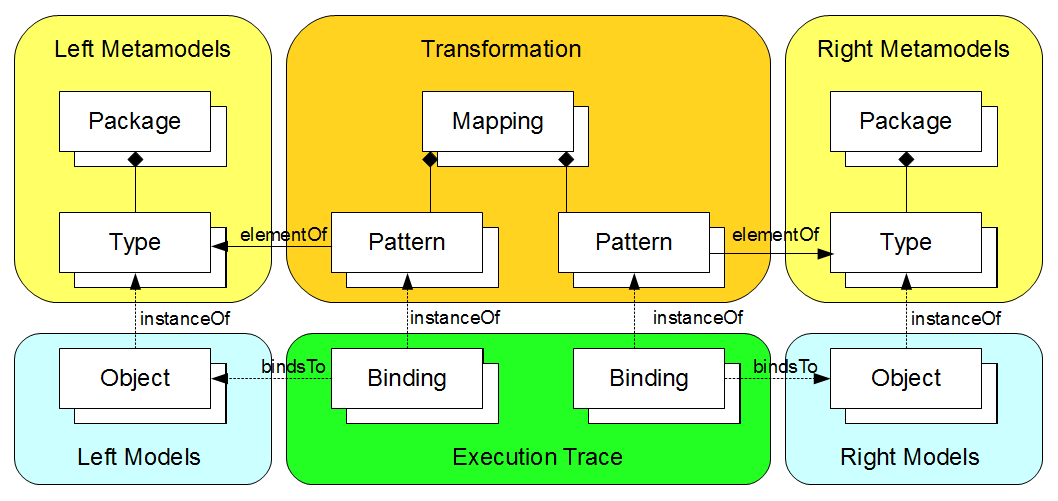
\includegraphics[width=0.45\textwidth]{TransformationAnatomy.png}
	\caption{Transformation Anatomy.}
	\label{fig:TransformationAnatomy}
\end{figure}

Since a declarative transformation expresses relationships to be satisfied, a transformation may be bi- or even multi-directional. The multi-directional capability allows a single transformation program to specify many model transformations, and to avoid the inconsistencies that may arise through writing independent programs for each direction and enforcement mode\footnote{check/create/update execution}.

In contrast an imperative transformation specifies the steps to obtain the target model from the source model for a single direction and enforcement\cite{Mens.Gorp2006}.

%Multi-directional transformations present several challenges, from an implementation point of view, in a number of domains and disciplines \cite{Czarnecki.etal2009}, some of which translate to QVT\cite{Stevens2010}. Declarative transformations present a challenge from a rule schedulability point of view. In the specific case of QVTr this translates to an implementation in which the execution of rules can be partial, interrupted or postponed until matches in other rules provide the required variable values (bindings), eventually requiring multiple passes. These challenges can be overcome by removing multi-directionality, normalizing constraints and defining an imperative semantics. 

The high level of abstraction of QVTr presents many specification and implementation challenges which the QVT \cite{QVT1.1} specification resolves with a QVTr to QVTc transformation. However although simpler, QVTc remains as powerful as QVTr but more verbose. The flexibilities of multi-directionality and the lack of an obvious execution schedule remain.

\begin{figure}[h]
	\centering
	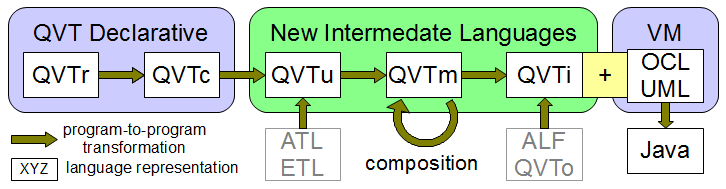
\includegraphics[width=0.45\textwidth]{QVThorizontalAlphabet.png}
	\caption{Overview of the proposed QVT 6 languages architecture.}
	\label{fig:overview}
\end{figure}

%QVTc is \textquotedblleft as powerful as the Relations language, though simpler. Consequently, the semantics of the Core Language can be defined more simply, though transformations described using the Core are more verbose\textquotedblright \cite{QVT1.1}. However, although having simpler semantics,  QVTc is still declarative and multi-directional and thus is difficult to implement. 

For efficient execution and more feasible implementation we propose a highly optimized unidirectional imperative language that we call QVT Imperative (QVTi). As with QVTr being realized by QVTc, QVTc can be realized by QVTi. Further, to facilitate this realization, we propose two additional languages QVT unidirectional (QVTu) and QVT minimal (QVTm) as presented in Figure \ref{fig:overview}. We propose a progressive program to program\footnote{We use program to program rather than model to model to stress the distinction between compile-time transformation of program models and run-time transformation of user models.} transformation chain
\begin{itemize}
\item QVTc to QVT unidirectional (QVTu); to align the transformation to the user's invocation context and eliminate the redundant multi-directional and enforcement flexibilities.
\item QVTu to QVT minimal (QVTm); to normalize the transformation to eliminate syntactic sugar and alternate representation flexibilities.
\item QVTm to QVT Imperative (QVTi); to discard declarative flexibilities and synthesize a multi-pass imperative search schedule that can be executed easily by a model-friendly Virtual Machine.
\end{itemize}

QVTi, QVTm and QVTu are simplifications of QVTc and so their meta-models are extensions of the OCL meta-model. An OCL execution facility such as the Eclipse OCL VM\cite{Willink2012} is therefore easily extended to support QVTi.

%For efficient execution and more feasible implementation we propose a highly optimized unidirectional imperative language that we call QVT Imperative (QVTi). The QVT specification's suggests that QVTr should be realized by a program-to-program transformation\footnote{We use program to program rather than model to model to stress the distinction between compile-time transformation of program models and run-time transformation of user models.} to QVTc (assuming an existing QVTc implementation). Following this approach QVTc will be realized by a program-to-program transformation to QVTi.

%However, the semantic gap between \textless multi-directional + declarative\textgreater\hspace{0pt} and \textless uni-directional + imperative\textgreater\hspace{0pt} makes it difficult to tackle the transformation in one step. Therefore, we propose two additional languages QVT unidirectional (QVTu) and QVT minimal (QVTm) as presented in Figure \ref{fig:overview}. Proximity of the QVTi syntax to EMOF and OCL will be useful as an AST interpretation and execution can be provided by extending the Eclipse OCL Virtual Machine\cite{Willink2012}.

%With a QVTi engine in place, and  we propose a program-to-program transformation from QVTc to QVTi. This transformation will be realized as a chain of three program-to-program transformations from QVTc to QVTu, QVTu to QVTm, and QVTm to QVTi. By also providing a QVTr to QVTc transformation we will be able to support QVTr.

These new languages also offer important interchange points for other transformation technologies to exploit and so share the tool chain in the future:

\begin{itemize}
\item QVTu provides a high level interchange point for other uni-directional declarative transformation languages such as ATL\cite{Jouault.etal2008} or ETL\cite{Paige.etal2009}.
\item QVTm provides a normalized representation at which declarative transformation composition and optimization can be applied.
\item QVTi provides a low level interchange point that imperative transformation languages such as QVTo, ALF\cite{Perseil2011} or EOL\cite{Paige.etal2009} may exploit.
\end{itemize}

%In short, we propose a top-down semantic simplification and a bottom-up implementation to eventually support the complete set of languages. In a future paper, we will discuss the details of the QVTu and QVTm languages and the QVTc to QVTi transformations. In this paper, we concentrate on the QVTi semantics and its derivation from QVTc, its execution and the reuse of QVTc concrete syntax for QVTi.

 %Moreover, there is a risk that what was gained from having to implement a simpler semantics would be lost by the work needed to realize the required transformation. Figure \ref{fig:overview} presents our progressive transformation solution to realizing QVTr on an OCL Virtual Machine\cite{Willink2012}. At the top we have the two QVT Declarative languages, with QVTr realized by a QVTr to QVTc program-to-program transformation. Our three new languages, QVTu, QVTm and QVTi are syntactic and semantic simplifications of QVTc.




%Since in QVTc the trace models must be explicitly defined, constraints are now defined by matching properties of elements in the candidate models and the trace models. Checking and enforcement provide the same functionality as in QVTr.

%The QVT specification states that the QVTr language supports complex object pattern matching (transformation rules) and defines its semantics in a combination of plan English and first order predicate logic. The complexity of the language semantics and the need to implicitly create and instantiate trace objects makes the implementation of QVTr a complex and daunting task.

%Trace classes used to record transformation execution are implicitly created. 



%three new languages, each one supporting a more restricted QVTc abstract syntax and providing increasingly limited semantics. QVTo operations will be invoked at the QVTi level and QVTi will provide an interface for QVTo to populate the middle (trace) model. 

%The intention of the QVTc subset languages is then to progressively restrict the QVTc semantics to eventually define a subset of QVTc that is uni-directional, normalized and imperative. The different levels of semantic \textquotedblleft power\textquotedblright will also imply a restriction on the use of the language's abstract syntax, from permissive to restricted. An overview of the proposed QVT alphabet is presented in Figure \ref{fig:overview}. 

%Complete support for QVTr is achieved by specifying mappings and implementing automated program transformations for:
%\begin{itemize}
%\item  QVTr$\rightarrow$QVTc, written in QVTc
%\item  QVTc$\rightarrow$QVTu, written in QVTu
%\item  QVTu$\rightarrow$QVTm, written in QVTm
%\item  QVTm$\rightarrow$QVTi, written in QVTi
%\end{itemize}








